\documentclass[c]{beamer}
\usetheme{default}
\title{Generalizing Nondeterminism for Algebraic Computation Machines}
\subtitle{Possible Subtitle}
\author{Scott Sanderson}
\institute{Department of Mathematics\\Williams College}
\date{\today}
\usepackage{tikz}
\usepackage{beamerthesiscommands}
\usepackage{mydiagrams}
\usepackage{graphicx}
% \usepackage{enumitem}
\usetikzlibrary{calc,arrows,shapes,positioning}

\begin{document}

\theoremstyle{definition}
\newtheorem{proposition}{Proposition}
\newtheorem{proofidea}{Proof Idea}

\begin{frame}
  \titlepage
\end{frame}

\begin{frame}{What is Complexity Theory?}
  
  \begin{columns}
    \visible<1->{
      \column{0.5\textwidth}
      \begin{figure}[h]
        \centering \scaletopagewidth{\algoyesno{}}
      \end{figure}
    }
    \visible<2->{
      \column{0.6\textwidth}
      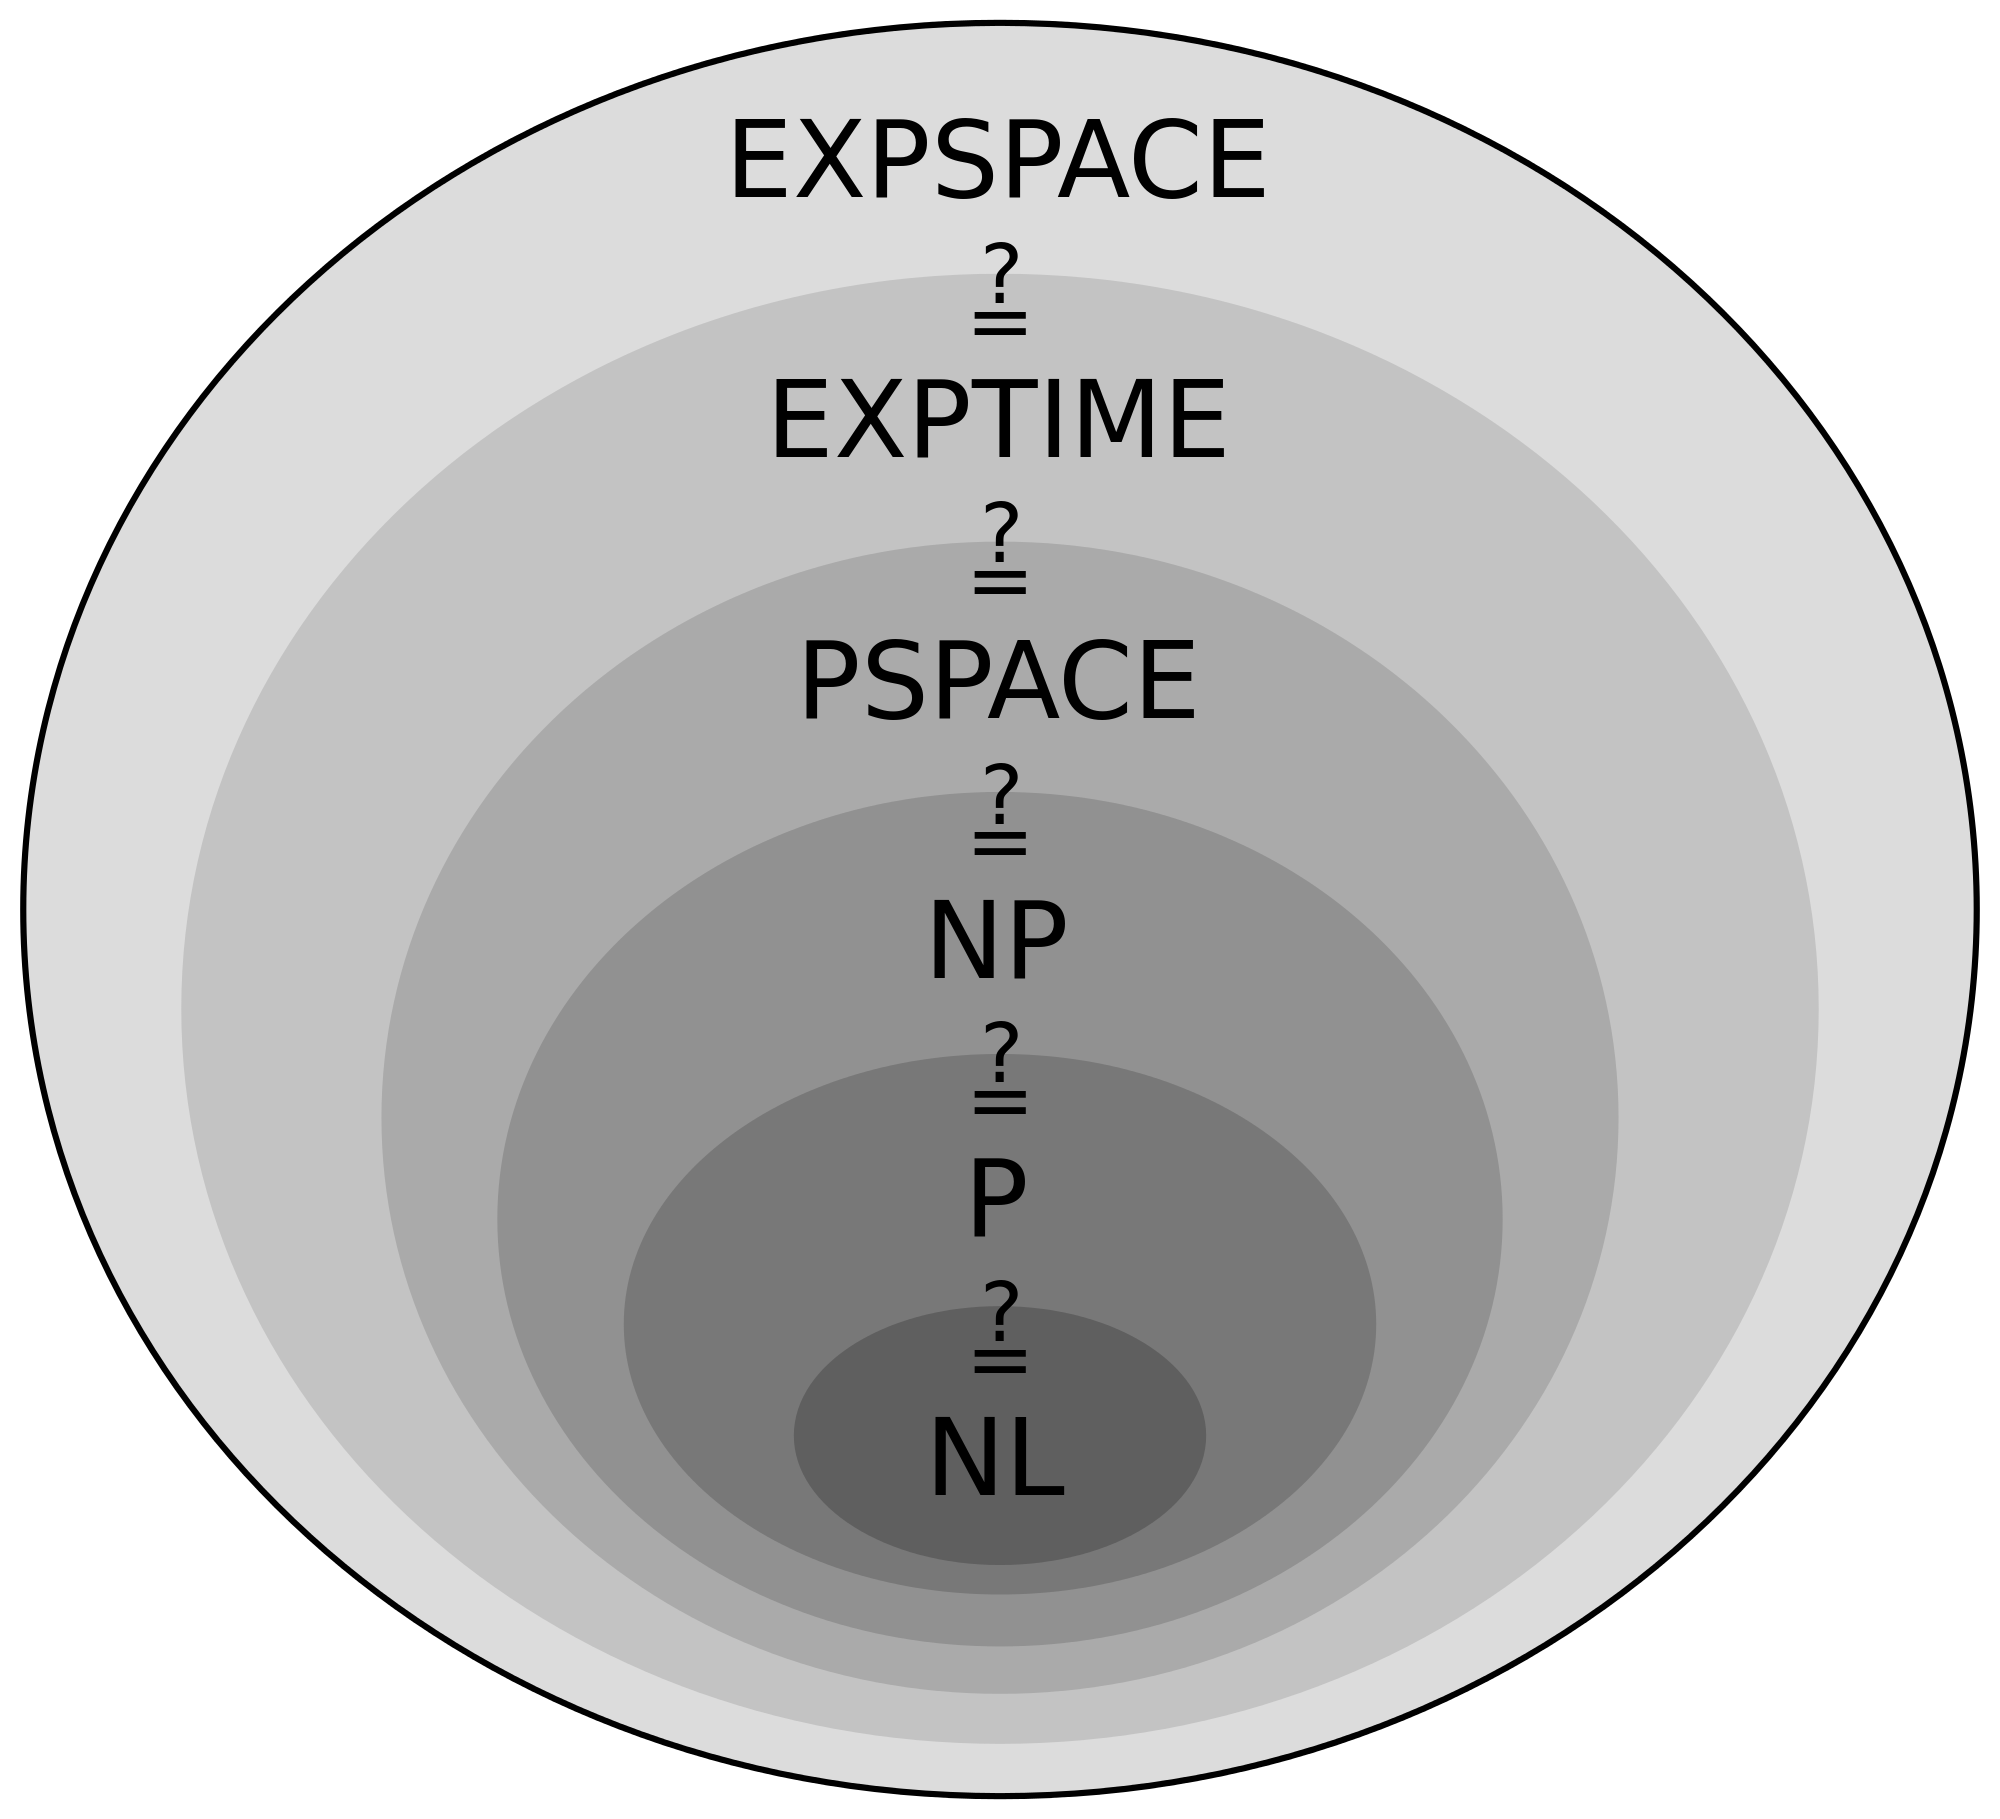
\includegraphics[width=\textwidth]{media/complexity.png}    
    }
  \end{columns}

\end{frame}

\begin{frame}{A Simple Puzzle}
  
  \begin{itemize}
  \item Does the set of numbers: $\set{1,4,7,-5,-3,18,-6,12}$ contain
    a subset adding up to 10? \pause
  \item Yes.  \textbf{Proof}: $18 - 3 - 6 + 1 = 10$ \pause
  \item Does $\set{1, 17, 25, -3, 11, -9, 22, 13}$ contain a subset
    adding up to $7$.\pause
  \item No.  \textbf{Proof}: Try them all! 
  \end{itemize}
  
\end{frame}

\begin{frame}{\subsum{}}

    An \textbf{instance} of \subsum{} is a pair $(S, t)$, where:

    \begin{itemize}
    \item $S = \set{s_1, s_2, \ldots, s_n}$ is a set of integers.
    \item $t$ is a single integer, called the \textbf{target} for $S$.
    \end{itemize}\pause

    An instance of \subsum{} is a \textbf{Yes Instance} if
    there exists some $X \subseteq S$ such that $\sum_X = t$.\\
    Otherwise it is a \textbf{No Instance}.\pause
\end{frame}

\begin{frame}{Decision Problems}

  \begin{itemize}
  \item \subsum{} is an example of what is known as a \textbf{Decision
      Problem}.\pause
  \item Very generally, a Decision Problem $D$ is a set of strings,
    partitioned into Yes Instances and No Instances, $D_{yes}$ and
    $D_{no}$.\pause
  \item The task associated with a Decision Problem is find a
    procedure for telling whether a given member of $D$ falls into
    $D_{yes}$ or $D_{no}$.\pause
  \item Computational Complexity Theory seeks to study the intrinsic
    \textbf{difficulty} of solving these tasks.
  \end{itemize}

\end{frame}

% \begin{frame}{Machine Models}
  
%   \begin{itemize}
%   \item We formalize the notion of ``procedure for performing a task''
%     by developing models of computing machines.\pause
%   \item In classical theory of computation, the de facto machine model
%     is the Turing Machine.
%   \end{itemize}

% \end{frame}

\begin{frame}{Turing Machine (Formal Definition)}

  \begin{definition}[Turing Machine (TM)]

    A \textbf{Turing Machine} is a 7-tuple, $(Q, \Sigma, \Gamma,
    \delta, q_0, q_{accept}, q_{reject})$, where:

    \begin{itemize}
    \item $Q$ is a set of machine states.
    \item $\Sigma$ is an alphabet of input characters, not containing
      the blank symbol, $\blank$.
    \item $\Gamma$ is the tape alphabet, with $\blank \in \Gamma$, and
      $\Sigma \subset \Gamma$.
    \item \functype{\delta}{(Q \times \Gamma)}{(Q \times \Gamma \times
        \set{L, R})} is the machine's
      \textbf{transition function}.
    \item $q_0$ is the initial state of the machine.
    \item $q_{accept}$ is the machine's accept state.
    \item $q_{reject}$ is the machine's reject state.
    \end{itemize}
  \end{definition}
  
\end{frame}

\begin{frame}{Turing Machines}
  \begin{columns}[c]

    \column{0.5\textwidth}
    \begin{itemize}
    \item Infinite one-dimensional tape, divided into cells.
    \item At each step, tape head reads a symbol, writes a symbol,
      moves left/right, and changes state.
    \item Tape head instructions encoded in a \textbf{transition
        function}.
    \end{itemize}
    \column{0.5\textwidth}
    \tape[1]{$q$}{{1,0,1,0,0,$\blank$, $\blank$, $\cdots$}}
    
  \end{columns}
\end{frame}

\begin{frame}{Turing Machine}

  \begin{itemize}
  \item Essentially, a Turing Machine is an infinite, one-way tape
    divided into cells, along with a tape head that rests on a
    single cell. \pause  
  \item The transition function $\delta$ encodes instructions
    which tell the tape head, at each step of the computation,
    write a symbol from $\Gamma$ to its current position, then
    move either left or right. \pause
  \item The specific instruction that gets executed depends on the
    state of the machine and the symbol currently under the tape
    head.\pause
  \item The machine halts and either \textbf{accepts} or
    \textbf{rejects} when it enters the special states $\qaccept$ or
    $\qreject$.

  \end{itemize}
\end{frame}

\begin{frame}[An Example Turing Machine Computation]
  \begin{columns}[c]
    
    \small

    \column{2in}

    \begin{itemize}
    \item $Q = \set{q_0, q_{accept}, q_{reject}}$
    \item $\Gamma = \set{\blank, 0, 1}$
    \item $\Sigma = \set{0,1}$
    \item $\delta(q_0, 0) = (q_0, 1, \rightarrow)$
    \item $\delta(q_0, 1) = (q_0, 0, \rightarrow)$
    \item $\delta(q_0, \blank) = (q_{accept}, \blank, \leftarrow)$
    \end{itemize}

    \column{2in}
    
    \begin{figure}[p]
      
      PLACEHOLDER
      
      %   \tape[1]{$q_0$}{{1,0,0,1,$\blank$,$\cdots$}} \vspace{1mm}
      %   \tape[2]{$q_0$}{{0,0,0,1,$\blank$,$\cdots$}} \vspace{1mm}
      %   \tape[3]{$q_0$}{{0,1,0,1,$\blank$,$\cdots$}} \vspace{1mm}
      %   \tape[4]{$q_0$}{{0,1,1,1,$\blank$,$\cdots$}} \vspace{1mm}
      %   \tape[5]{$q_0$}{{0,1,1,0,$\blank$,$\cdots$}} \vspace{1mm}
      %   \tape[4]{$q_{accept}$}{{0,1,1,0,$\blank$, $\cdots$}} \vspace{1mm}
      % \caption{An Example Turing Machine Computation}
    \end{figure}
    
  \end{columns}
\end{frame}

\begin{frame}{Limitations of Turing Machines}

  \begin{itemize}
  \item The computation of a Turing Machine only makes sense for
    inputs that are representable by finite sequences of characters
    drawn from finite alphabet. \pause
  \item This means we can't talk about problems that are naturally
    defined over uncountable sets, such as $\reals$ or $\complexes$.\pause
  \item A natural example of such a problem is the Mandelbrot Set
    $\mathcal{M}$
  \end{itemize}
  
\end{frame}

\begin{frame}{The Mandelbrot Set $\mathcal{M}$}
  
  Let $c \in \complexes$, we define:
    \begin{align*}
      p_c(z) &= z^2 + c\\
      p_c^n(z) &= p_c(\ldots(p_c(p_c(z)))) \text{ $n$ times }\\
    \end{align*}
    \vspace{-\baselineskip}
    
    The Mandelbrot Set $\mathcal{M}$ is given by:
    $$\set{c \in \complexes |p_c^n(0) \nrightarrow \infty \text{ as } n \rightarrow \infty}$$
    
\end{frame}

\begin{frame}{The Mandelbrot Set $\mathcal{M}$}
  \begin{columns}

    \column[c]{0.3\textwidth}
    {\scriptsize
    $$c = 0.5 + 0.5i$$
    \begin{align*}
      p_c(0) &=& 0.5 + 0.5i\\
      p_c(p_c(0)) &=& 0.5 + i\\
      p_c(p_c(p_c(0))) &=& -.25 + 1.5i\\
      p_c^4(0) &=& -1.687 + -.25i\\
      p_c^5(0) &=& 3.285 + 1.34i\\
    \end{align*}
    }
    \column{0.7\textwidth}
    \begin{center}
      \scaletopagewidth{
        \begin{tikzpicture}[>=latex']
          \draw [thick] (-3.0,0) -- (3.0,0); 
          \draw [thick](0,-3.0) --  (0,3.0); 
          \draw (0,0) circle (2.0cm); 
          \node (start) [mandpoint] at (0.0, 0.0) {};
          \node (p0) [mandpoint] at (0.5, 0.5) {};
          \node (p1) [mandpoint] at (0.5, 1) {};
          \node (p2) [mandpoint] at (-0.25, 1.5) {};
          \node (p3) [mandpoint] at (-1.6875, -.25) {};
          \node (p4) [mandpoint] at (3.285, 1.343) {};

          % \draw [->] (start) edge[out=
          \draw [->] (p0) edge[out=90, in=270] (p1);
          \draw [->] (p1) edge[out=90, in=0] (p2);
          \draw [->] (p2) edge[out=180, in=90] (p3);
          \draw [->] (p3) edge[out=0, in=270] (p4);

        \end{tikzpicture}
      }
    \end{center}

  \end{columns}
\end{frame}

\begin{frame}{The Mandelbrot Set $\mathcal{M}$}

  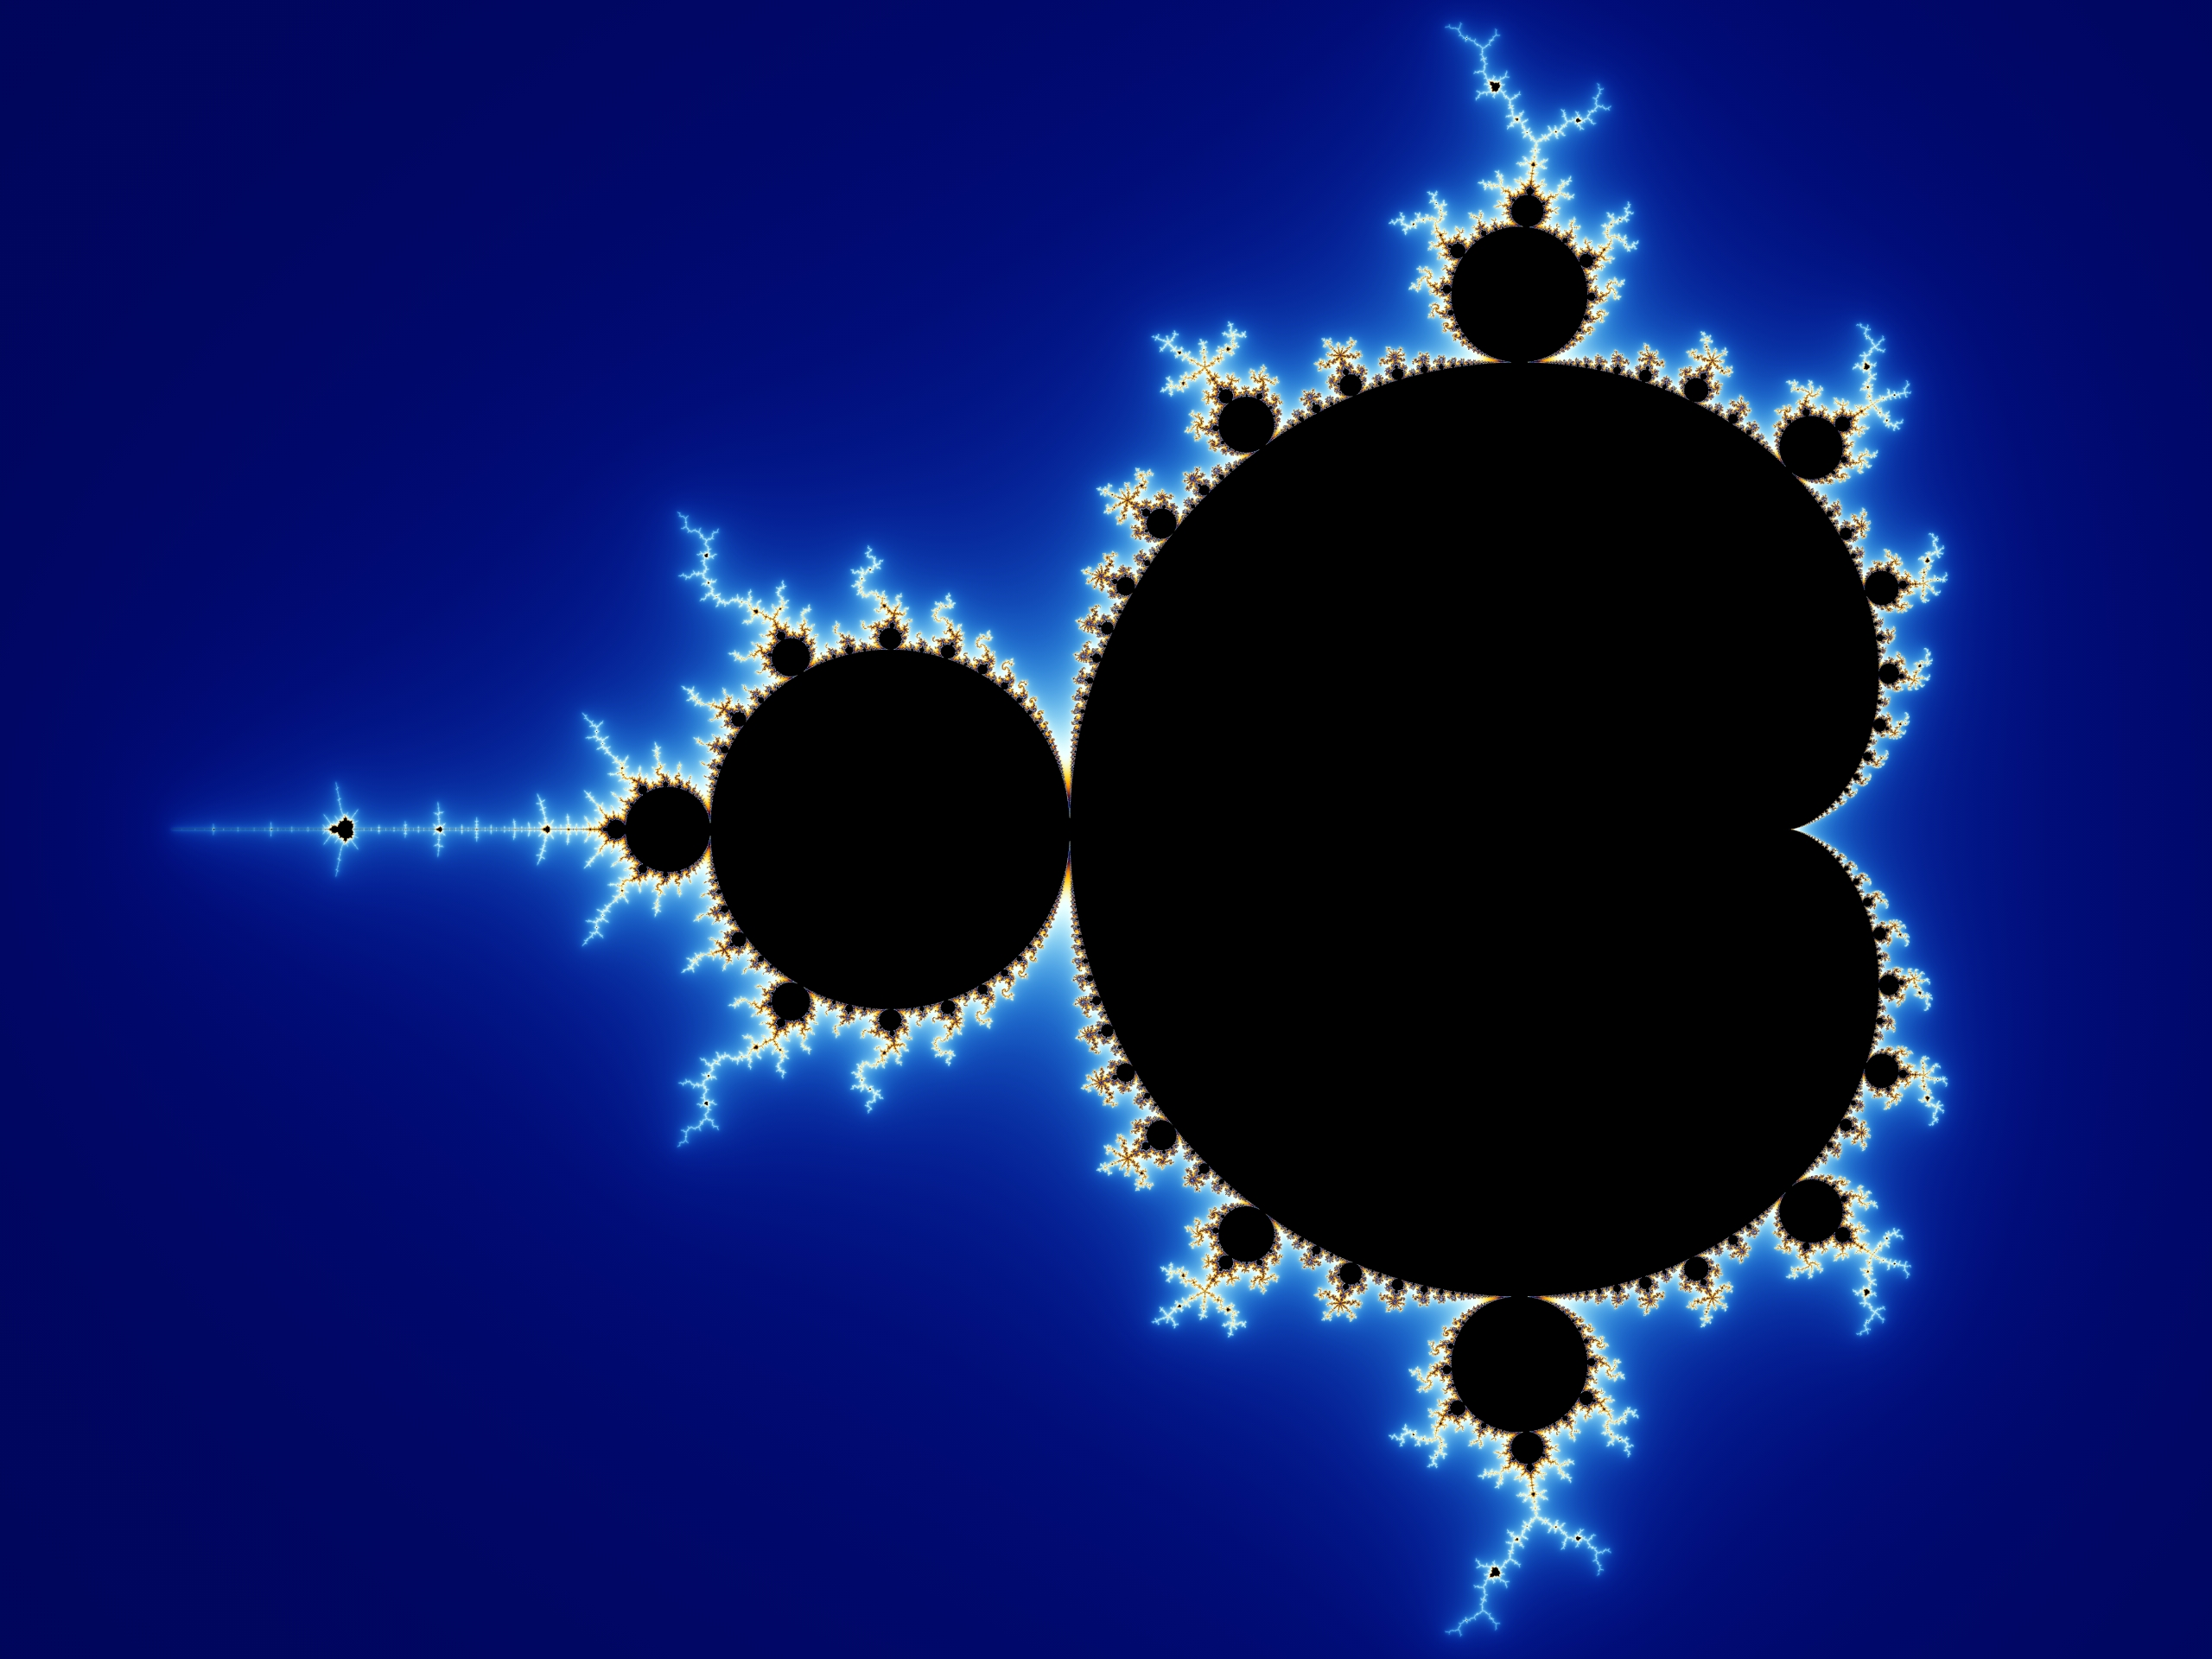
\includegraphics[width=\textwidth]{media/mandelbrot.jpg}
  
\end{frame}

\begin{frame}{The Mandelbrot Set as Decision Problem}
  
  \begin{itemize}
  \item In general it's easy to tell if some $c \in \complexes$ is
    \textbf{not} in the Mandelbrot Set.\pause
  \item If at any point in computing the sequence $p_c(0),
    p_c(p_c(0)), \ldots$ we see a value greater than 2, it is
    guaranteed to escape to infinity, so it can't be in
    $\mathcal{M}$\pause
  \item It seems harder to find a condition such that a complex number
    $c$ is guaranteed \textbf{not} to escape to infinity.
  \end{itemize}
\end{frame}

\begin{frame}{The Mandelbrot Set as Decision Problem}
  
  \textbf{Question}: Does there exist an algorithm for determining
  whether an arbitrary complex number $c$ is a member of
  $\mathcal{M}$?
  
\end{frame}

\begin{frame}{Finite Dimensional BSS Machines}

  PLACEHOLDER
  
\end{frame}

\begin{frame}{Finite Dimensional BSS Machines}

  PLACEHOLDER
  
\end{frame}

\begin{frame}{Example FDM}
  
  PLACEHOLDER (Mandelbrot Set Decider over C)
 
\end{frame}

\begin{frame}{Example FDM}
  
  PLACEHOLDER (Rational recognizer over R)
 
\end{frame}

\begin{frame}{Path Decomposition Theorem}

  PLACEHOLDER (State, give proof idea, maybe talk about computation
  paths/coincidence sets?)
  
\end{frame}

\begin{frame}
  \begin{corollary}
    The Mandelbrot Set is undecidable.
  \end{corollary}
\end{frame}

\begin{frame}{``Full'' BSS Machines}

  PLACEHOLDER

\end{frame}




\end{document}